\section{Fundamento teórico}

Para comenzar se deben establecer unos parámetros para con la pala, ya que lo más básico de este trabajo empieza por determinar los efectos que produce la torsión en nuestra obtención de energía.

Es por ello que se determina que la pala de la turbina eólica es un \textbf{trapecio} cuya representación simplificada la vemos en la Figura \ref{fig:pala_simp}


\begin{figure}[H]
    \centering
    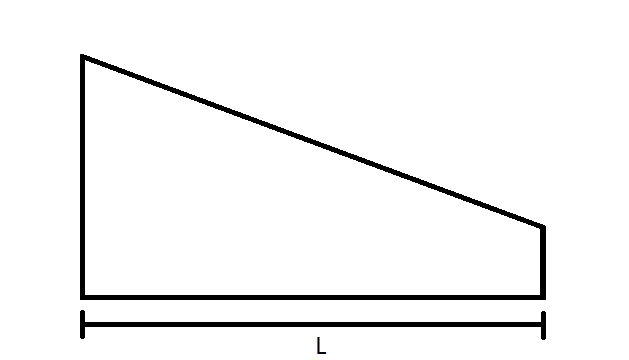
\includegraphics[width=0.7\textwidth]{images/pala turbina paint.png}
    \caption{Representación de una pala de turbina eólica}
    \textit{Fuente: Elaboración propia}
    \label{fig:pala_simp}
\end{figure}



Lo siguiente que se debe tener presente es que se necesita también una representación de la pala de la figura \ref{fig:pala_simp} dividida en segmentos de igual largo para poder comprender el desarrollo que se realizará simulando una torsión, en la cual se girarán los segmentos un cierto ángulo los unos de los otros.

    \textbf{}
    \begin{figure}[H]
    \centering
    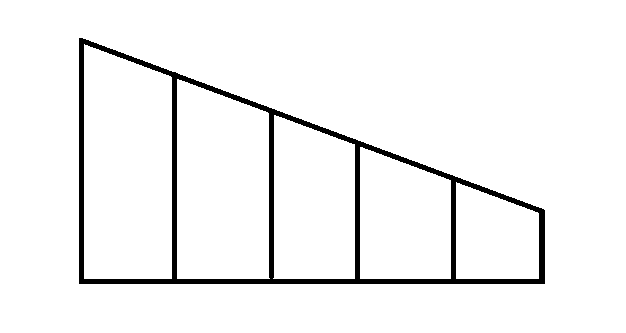
\includegraphics[width=0.7\textwidth]{images/pala dividida.png}
    \caption{Representación de una pala de turbina eólica en segmentos}
    \textit{Fuente: Elaboración propia}
    \label{fig:pala_dividida}
\end{figure}

Por simplicidad, la pala se dividirá únicamente en $N$ segmentos, en este caso 5. Aunque se mantenga este valor durante el trabajo y es probable que no cambie, se asociará a una variable en caso de que se quieran hacer pruebas mediante simulación en MATLAB más adelante. \\\\
    

La $L$ o \textit{longitud de pala}, vista en la Figura \ref{fig:pala_simp} es con la que se va a trabajar, por ello cada uno de los segmentos de la Figura \ref{fig:pala_dividida} tendrá el siguiente largo $\dfrac{L}{N} = \dfrac{L}{5}$ ya que se dividió $N$ número de veces. \\

Como se puede observar en la Figura \ref{fig:pala_dividida} cada segmento tiene una altura variable, esto se debe a la forma real de las palas, cuanto más cerca del buje de la turbina, mayor es el área del segmento. La altura en el centro de estos segmentos, conocida como $chord \text{ } line$ o $línea \text{ } de \text{ } cuerda$ se determinará mediante el preestablecimiento de una serie de datos y su desarrollo matemático relacionados con la pala completa.\\

Para el cálculo de la $línea \text{ } de \text{ } cuerda$ se requiere la realización de un desarrollo trigonométrico. 

\begin{figure}[H]
    \centering
    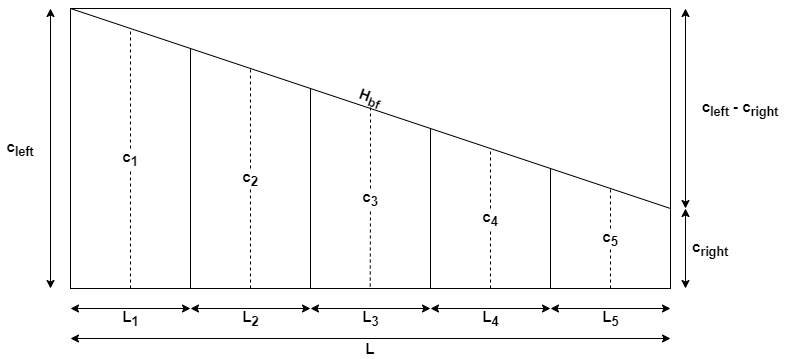
\includegraphics[width=0.9\textwidth]{images/planteo chord line.png}
    \caption{Representación parametrizada de la pala de una turbina eólica marina}
    \textit{Fuente: Elaboración propia}
    \label{fig:pala_desarrollo_chord}
\end{figure}



\begin{definicion}
En base a esta representación esquemática se puede deducir que:
$$ c_{left} = J$$
$$ c_{right} = J/D$$
$$ L_i = L/N$$
Donde,
\centering
J y D $\in \mathbb{Q+}$, \hspace{2pt} $J > D$, \hspace{2pt} $L_i$ := longitud del segmento,  $c_{left}$ := longitud simplificada del buje o hub de la pala y $c_{right}$ := longitud simplificada de la punta o tip de la pala, $i \in segmento$ y $segmento = \{1, ..., N\}$ 
\label{def_laterales_pala}
\end{definicion}


Ahora, una vez se tienen las variables básicas para conocer el resto de parámetros, se comienza con los cálculos.

\begin{definicion}
Con las variables formalizadas en la anterior definición, se define el valor $H_{bf}$ mediante el teorema de Pitágoras ya que el triángulo es rectángulo.

$$ H_{bf} = \sqrt{(c_{left} - c_{right})^{2} + L^{2}}$$
Donde,
\centering
$L$ := longitud de la pala, $H_{bf}$ := borde de fuga de la pala, $c_{left}$ := longitud simplificada del buje o hub de la pala y $c_{right}$ := longitud simplificada de la punta o tip de la pala.
\label{def_hipotenusa_pala}
\end{definicion}


A continuación, lo próximo que se debe obtener es el ángulo $\Phi$ o \textit{Ángulo de la línea del borde de arrastre de la pala de la turbina eólica}, para así conocer como decrece la $H_{bf}$ y mediante una relación trigonométrica extraída del artículo \cite{armenta2021predictive} poder obtener los valores de la \textit{Líneas de cuerda}.

\begin{figure}[H]
    \centering
    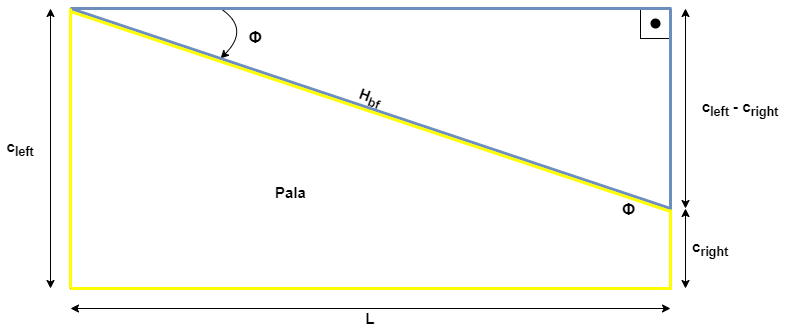
\includegraphics[width=0.9\textwidth]{images/triangulo sacar phi.drawio.png}
    \caption{Pala de la turbina en amarillo y triángulo usado para el cálculo de $\Phi$ en azul}
    \textit{Fuente: Elaboración propia}
    \label{fig:pala_calculo_phi}
\end{figure}

\begin{definicion}
En base a la figura \ref{fig:pala_calculo_phi} se puede deducir de tres formas por trigonometría el ángulo $\Phi$:
$$ \Phi = \arcsin{(\dfrac{c_{left} - c_{right}}{H_{bf}})} $$
$$ \Phi = \arccos{(\dfrac{L}{H_{bf}})} $$
$$ \Phi = \arctan{( \dfrac{\sin{(\dfrac{c_{left} - c_{right}}{H_{bf}})}}{\cos{(\dfrac{L}{H_{bf}})}} ) } $$
Donde,
\centering
$L$ := longitud de la pala, $H_{bf}$ := borde de fuga de la pala, $c_{left}$ := longitud simplificada del buje o hub de la pala y $c_{right}$ := longitud simplificada de la punta o tip de la pala.
\label{def_angulo_phi}
\end{definicion}


El siguiente paso para calcular las $líneas \text{ } de \text{ } cuerda$ se basa en aislar trapecios mas pequeños de los que se han obtenido todos los datos menos el valor de su base menor que se tendrá que calcular, siendo este equivalente a $c$.\\

\begin{definicion}
Variables necesarias para el cálculo de las líneas de cuerda.

$$ altura_i = \dfrac{(2i - 1) \cdot L}{2N}$$
$$ diagonal_i = \dfrac{(2i - 1) \cdot H_{bf}}{2N}$$

Donde,
\centering
$L$ := longitud de la pala, $H_{bf}$ := borde de fuga de la pala, $altura_i$ := Longitud de la pala fragmentada para el cálculo de la línea de cuerda, $H_{bf}$ := Hipotenusa del borde de fuga fragmentada para el cálculo de la línea de cuerda, $i \in segmento$ y $segmento = \{1, ..., N\}$
\label{def_variables_fragmentadas}
\end{definicion}

Por último y una vez definido todo lo necesario, se pasa al cálculo mediante el cual se obtiene el valor de todas y cada una de las $líneas \text{ } de \text{ } cuerda$ de la pala con la que se está trabajando.

\begin{definicion}
Primero se obtiene la diferencia mediante Pitágoras entre la base mayor y la menor, definida como $x_i$, después la resta de la base mayor y esta diferencia.

$$ x_i = \sqrt{diagonal_i^{2} - altura_i^{2}}$$

$$ c_i = c_{left} - x_i $$

Donde,
\centering
$L$ := longitud de la pala, $H_{bf}$ := borde de fuga de la pala, $altura_i$ := Longitud de la pala fragmentada para el cálculo de la línea de cuerda, $H_{bf}$ := Hipotenusa del borde de fuga fragmentada para el cálculo de la línea de cuerda, $i \in segmento$ y $segmento = \{1, ..., N\}$
\label{def_chord_line}
\end{definicion}

% Ahora, debería determinar los c_right y c_left de todos y cada uno de los segmentos para poder calcular su área mediante el desarrollo de nuestro amigo y vecino carlos. De esa manera se podrá usar en la ristra de fórmulas que tengo en el otro lado.